\documentclass{standalone}
\usepackage{tikz}
\usetikzlibrary{patterns, positioning}


\begin{document}
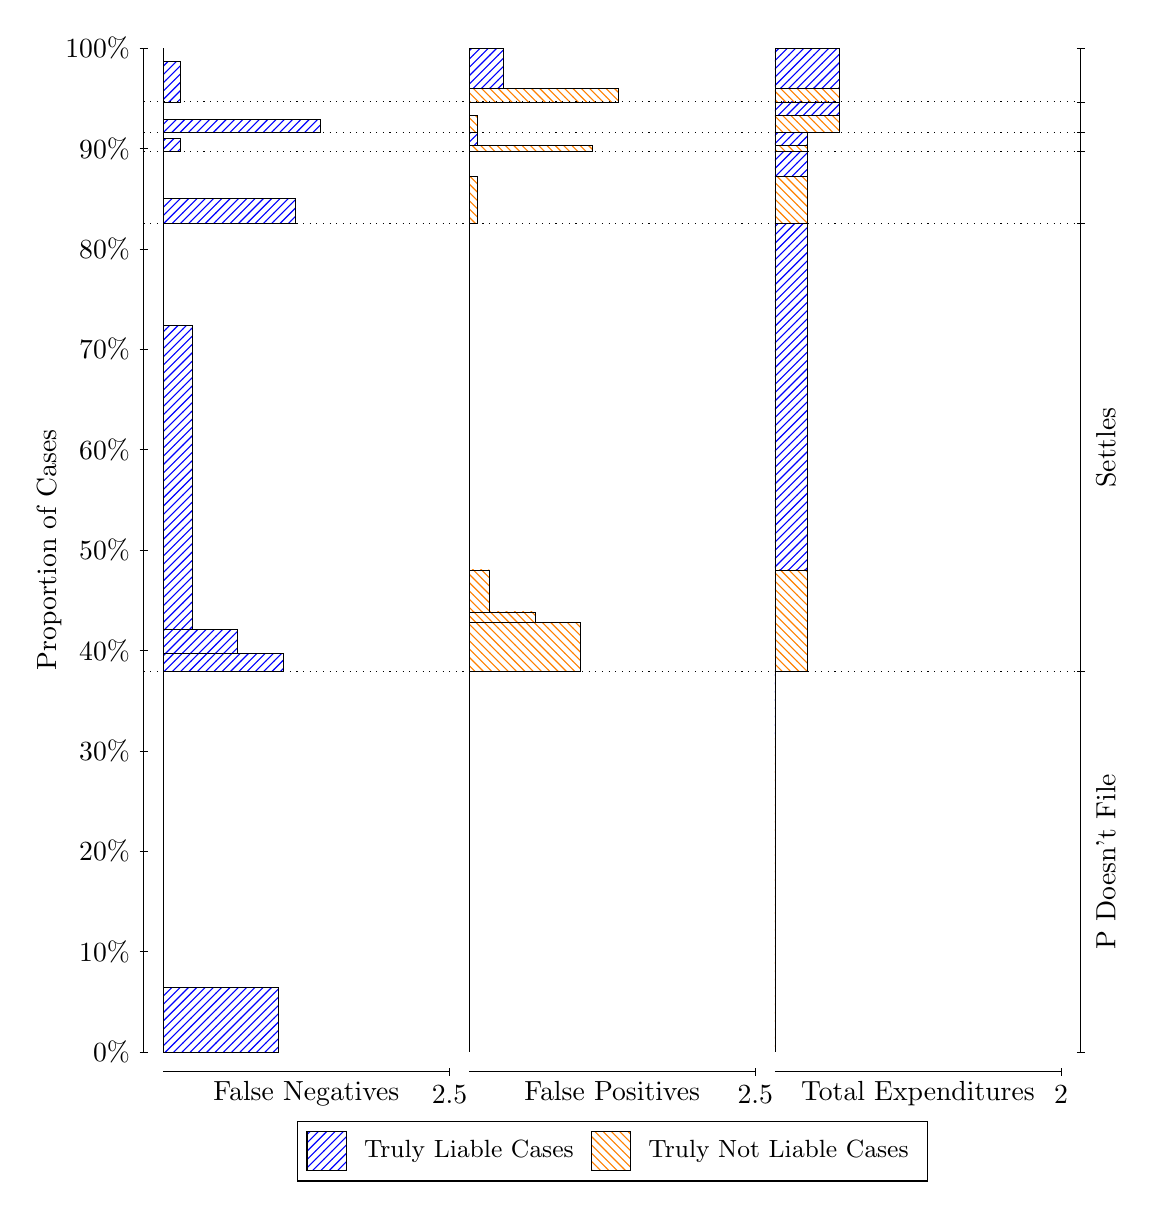
\begin{tikzpicture}
\draw[black, very thin] (1.5,1.75) -- (1.5,14.5);
\node[rotate=90, text=black, anchor=center] at (0.3, 8.125) {Proportion of Cases};
\draw[black, very thin] (1.45,1.75) -- (1.55,1.75);
\node[text=black, anchor=east] at (1.45, 1.75) {0\%};
\draw[black, very thin] (1.45,3.025) -- (1.55,3.025);
\node[text=black, anchor=east] at (1.45, 3.025) {10\%};
\draw[black, very thin] (1.45,4.3) -- (1.55,4.3);
\node[text=black, anchor=east] at (1.45, 4.3) {20\%};
\draw[black, very thin] (1.45,5.575) -- (1.55,5.575);
\node[text=black, anchor=east] at (1.45, 5.575) {30\%};
\draw[black, very thin] (1.45,6.85) -- (1.55,6.85);
\node[text=black, anchor=east] at (1.45, 6.85) {40\%};
\draw[black, very thin] (1.45,8.125) -- (1.55,8.125);
\node[text=black, anchor=east] at (1.45, 8.125) {50\%};
\draw[black, very thin] (1.45,9.4) -- (1.55,9.4);
\node[text=black, anchor=east] at (1.45, 9.4) {60\%};
\draw[black, very thin] (1.45,10.675) -- (1.55,10.675);
\node[text=black, anchor=east] at (1.45, 10.675) {70\%};
\draw[black, very thin] (1.45,11.95) -- (1.55,11.95);
\node[text=black, anchor=east] at (1.45, 11.95) {80\%};
\draw[black, very thin] (1.45,13.225) -- (1.55,13.225);
\node[text=black, anchor=east] at (1.45, 13.225) {90\%};
\draw[black, very thin] (1.45,14.5) -- (1.55,14.5);
\node[text=black, anchor=east] at (1.45, 14.5) {100\%};

\draw[black, very thin] (13.4,1.75) -- (13.4,14.5);
\draw[black, very thin] (13.35,1.75) -- (13.45,1.75);
\node[anchor=west] at (13.35, 1.75) {};
\draw[black, very thin] (13.35,6.5816) -- (13.45,6.5816);
\node[anchor=west] at (13.35, 6.5816) {};
\draw[black, very thin] (13.35,12.271) -- (13.45,12.271);
\node[anchor=west] at (13.35, 12.271) {};
\draw[black, very thin] (13.35,13.189) -- (13.45,13.189);
\node[anchor=west] at (13.35, 13.189) {};
\draw[black, very thin] (13.35,13.424) -- (13.45,13.424);
\node[anchor=west] at (13.35, 13.424) {};
\draw[black, very thin] (13.35,13.817) -- (13.45,13.817);
\node[anchor=west] at (13.35, 13.817) {};
\draw[black, very thin] (13.35,14.5) -- (13.45,14.5);
\node[anchor=west] at (13.35, 14.5) {};

\draw[black, very thin, pattern color=blue, pattern=north east lines] (1.75,1.75) rectangle (3.2033,2.5671);
\draw[black, very thin, pattern color=orange, pattern=north west lines] (1.75,2.5671) rectangle (1.75,6.5816);
\draw[black, very thin, pattern color=blue, pattern=north east lines] (1.75,6.5816) rectangle (3.276,6.8144);
\draw[black, very thin, pattern color=blue, pattern=north east lines] (1.75,6.8144) rectangle (2.6947,7.1166);
\draw[black, very thin, pattern color=blue, pattern=north east lines] (1.75,7.1166) rectangle (2.1133,10.979);
\draw[black, very thin, pattern color=orange, pattern=north west lines] (1.75,10.979) rectangle (1.75,12.271);
\draw[black, very thin, pattern color=blue, pattern=north east lines] (1.75,12.271) rectangle (3.4213,12.586);
\draw[black, very thin, pattern color=orange, pattern=north west lines] (1.75,12.586) rectangle (1.75,13.189);
\draw[black, very thin, pattern color=blue, pattern=north east lines] (1.75,13.189) rectangle (1.968,13.352);
\draw[black, very thin, pattern color=orange, pattern=north west lines] (1.75,13.352) rectangle (1.75,13.424);
\draw[black, very thin, pattern color=blue, pattern=north east lines] (1.75,13.424) rectangle (3.7483,13.594);
\draw[black, very thin, pattern color=orange, pattern=north west lines] (1.75,13.594) rectangle (1.75,13.817);
\draw[black, very thin, pattern color=blue, pattern=north east lines] (1.75,13.817) rectangle (1.968,14.329);
\draw[black, very thin, pattern color=orange, pattern=north west lines] (1.75,14.329) rectangle (1.75,14.5);
\draw[black, very thin, pattern color=orange, pattern=north west lines] (5.6333,1.75) rectangle (5.6333,5.7645);
\draw[black, very thin, pattern color=blue, pattern=north east lines] (5.6333,5.7645) rectangle (5.6333,6.5816);
\draw[black, very thin, pattern color=orange, pattern=north west lines] (5.6333,6.5816) rectangle (7.0503,7.2044);
\draw[black, very thin, pattern color=orange, pattern=north west lines] (5.6333,7.2044) rectangle (6.469,7.3384);
\draw[black, very thin, pattern color=orange, pattern=north west lines] (5.6333,7.3384) rectangle (5.8877,7.8734);
\draw[black, very thin, pattern color=blue, pattern=north east lines] (5.6333,7.8734) rectangle (5.6333,12.271);
\draw[black, very thin, pattern color=orange, pattern=north west lines] (5.6333,12.271) rectangle (5.7423,12.874);
\draw[black, very thin, pattern color=blue, pattern=north east lines] (5.6333,12.874) rectangle (5.6333,13.189);
\draw[black, very thin, pattern color=orange, pattern=north west lines] (5.6333,13.189) rectangle (7.1957,13.26);
\draw[black, very thin, pattern color=blue, pattern=north east lines] (5.6333,13.26) rectangle (5.7423,13.424);
\draw[black, very thin, pattern color=orange, pattern=north west lines] (5.6333,13.424) rectangle (5.7423,13.647);
\draw[black, very thin, pattern color=blue, pattern=north east lines] (5.6333,13.647) rectangle (5.6333,13.817);
\draw[black, very thin, pattern color=orange, pattern=north west lines] (5.6333,13.817) rectangle (7.5227,13.988);
\draw[black, very thin, pattern color=blue, pattern=north east lines] (5.6333,13.988) rectangle (6.0693,14.5);
\draw[black, very thin, pattern color=orange, pattern=north west lines] (9.5167,1.75) rectangle (9.5167,5.7645);
\draw[black, very thin, pattern color=blue, pattern=north east lines] (9.5167,5.7645) rectangle (9.5167,6.5816);
\draw[black, very thin, pattern color=orange, pattern=north west lines] (9.5167,6.5816) rectangle (9.9254,7.8734);
\draw[black, very thin, pattern color=blue, pattern=north east lines] (9.5167,7.8734) rectangle (9.9254,12.271);
\draw[black, very thin, pattern color=orange, pattern=north west lines] (9.5167,12.271) rectangle (9.9254,12.874);
\draw[black, very thin, pattern color=blue, pattern=north east lines] (9.5167,12.874) rectangle (9.9254,13.189);
\draw[black, very thin, pattern color=orange, pattern=north west lines] (9.5167,13.189) rectangle (9.9254,13.26);
\draw[black, very thin, pattern color=blue, pattern=north east lines] (9.5167,13.26) rectangle (9.9254,13.424);
\draw[black, very thin, pattern color=orange, pattern=north west lines] (9.5167,13.424) rectangle (10.334,13.647);
\draw[black, very thin, pattern color=blue, pattern=north east lines] (9.5167,13.647) rectangle (10.334,13.817);
\draw[black, very thin, pattern color=orange, pattern=north west lines] (9.5167,13.817) rectangle (10.334,13.988);
\draw[black, very thin, pattern color=blue, pattern=north east lines] (9.5167,13.988) rectangle (10.334,14.5);
\draw[black, dotted] (1.5,6.5816) -- (13.4,6.5816);
\draw[black, dotted] (1.5,12.271) -- (13.4,12.271);
\draw[black, dotted] (1.5,13.189) -- (13.4,13.189);
\draw[black, dotted] (1.5,13.424) -- (13.4,13.424);
\draw[black, dotted] (1.5,13.817) -- (13.4,13.817);
\draw[black, very thin] (1.75,1.5) -- (5.3833,1.5);
\node[text=black, anchor=north] at (3.5667, 1.5) {False Negatives};
\draw[black, very thin] (5.3833,1.45) -- (5.3833,1.55);
\node[text=black, anchor=north] at (5.3833, 1.45) {2.5};

\draw[black, very thin] (5.6333,1.5) -- (9.2667,1.5);
\node[text=black, anchor=north] at (7.45, 1.5) {False Positives};
\draw[black, very thin] (9.2667,1.45) -- (9.2667,1.55);
\node[text=black, anchor=north] at (9.2667, 1.45) {2.5};

\draw[black, very thin] (9.5167,1.5) -- (13.15,1.5);
\node[text=black, anchor=north] at (11.333, 1.5) {Total Expenditures};
\draw[black, very thin] (13.15,1.45) -- (13.15,1.55);
\node[text=black, anchor=north] at (13.15, 1.45) {2};

\node[text=black, centered, rotate=90] at (13.72, 4.1658) {P Doesn't File};
\node[text=black, centered, rotate=90] at (13.72, 9.4264) {Settles};





\draw (7.449999999999999,1.5) node[draw=none] (baseCoordinate) {};
\begin{scope}[align=center]
        \matrix[scale=0.5, draw=black, below=0.5cm of baseCoordinate, nodes={draw}, column sep=0.1cm]{
            \node[rectangle, draw, minimum width=0.5cm, minimum height=0.5cm, pattern color=blue, pattern=north east lines] {}; &
            \node[draw=none, font=\small, text=black] (B) {Truly Liable Cases}; &
            \node[rectangle, draw, minimum width=0.5cm, minimum height=0.5cm, pattern color=orange, pattern=north west lines] {}; &
            \node[draw=none, font=\small, text=black] (B) {Truly Not Liable Cases}; \\
            };
\end{scope}

\end{tikzpicture}
\end{document}